\begin{blocksection}
\question What would Python display? Follow the series of function calls. What are g and h assigned to after running the code? (Recommended: Draw an environment diagram!)

\begin{lstlisting}
>>> def f(x, y):
...   x, y = y, x
...   def x(x):
...     return y(x)
...   return x
...
>>> def y(x):
...   return 6 + x
...
>>> def z(y):
...   return 4
... 
>>> g = f(y, z)
>>> h = g(5)
\end{lstlisting}

\begin{solution}
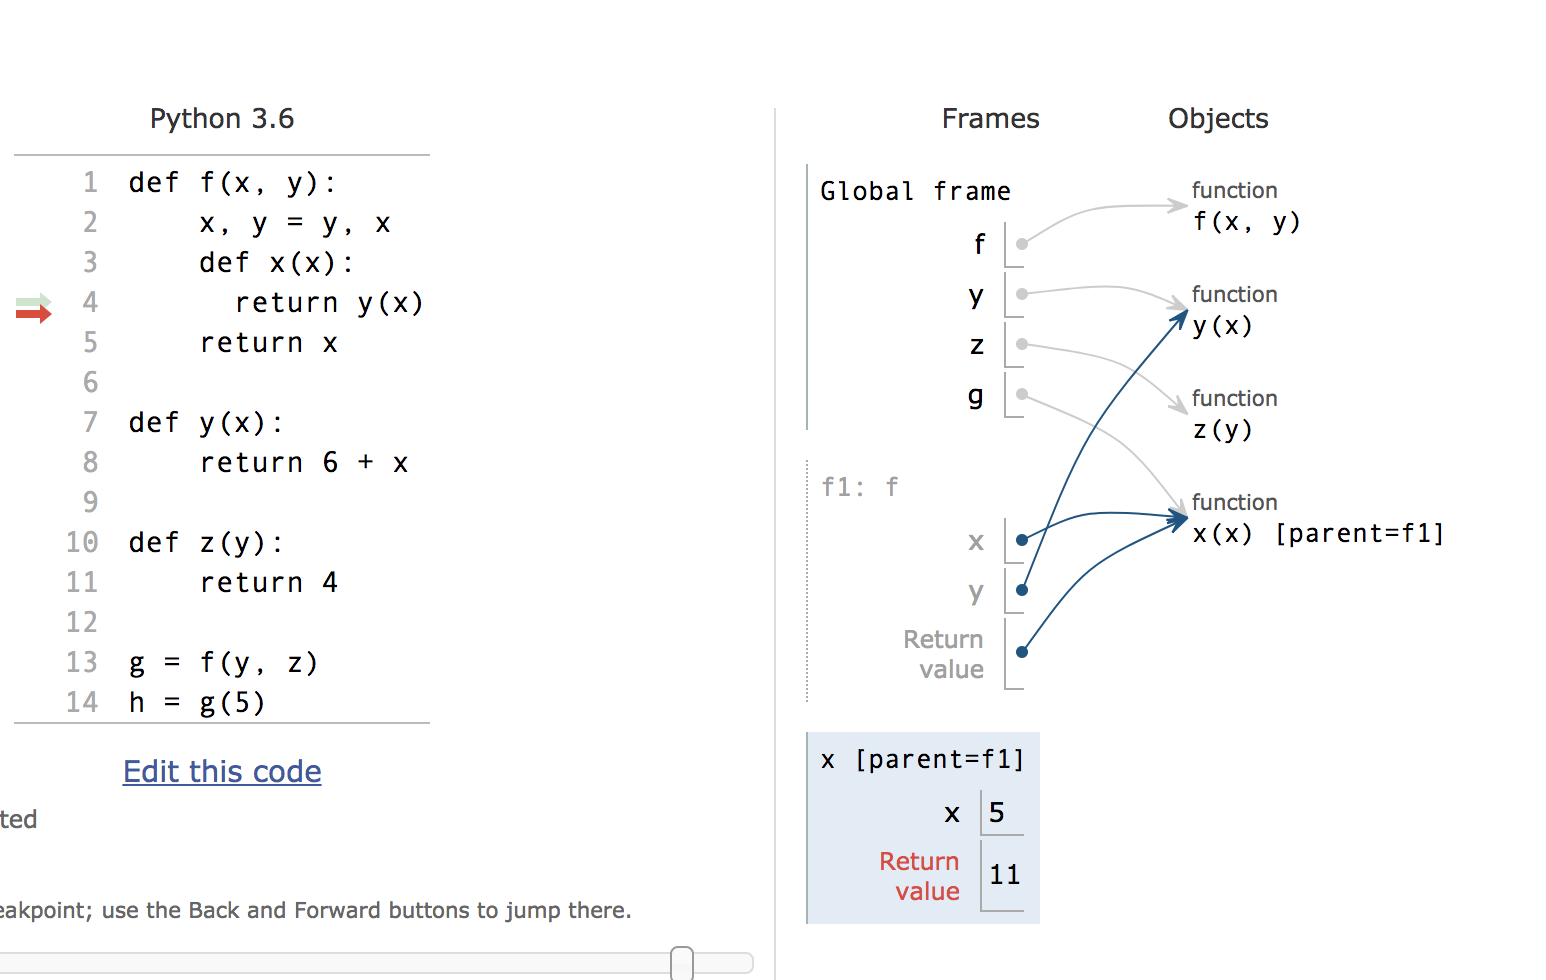
\includegraphics[scale=0.5]{fxyz.png}
\newline
\url{https://goo.gl/B7dFTh}
\end{solution}
\end{blocksection}
